% DIN A4 has height 297mm (792pt) % and width 210mm (560pt).
% 1pt is 0.375mm

\documentclass[paper=a4,11pt,oneside]{article}
\usepackage[headinclude]{typearea}

% language and encoding
\usepackage[ngerman]{babel} 
% Deutsch und Englisch
\usepackage[ansinew]{inputenc}
% improve text rendering
\usepackage[final,protrusion=true,expansion=false]{microtype}

% graphics
\usepackage[table,hyperref,svgnames,x11names]{xcolor}
\usepackage{graphicx}
\usepackage{tikz}
\usetikzlibrary{plotmarks}
\usepackage{pgfplots}
\pgfplotsset{compat=1.16}

% math
\usepackage{mathtools}
\usepackage{amsthm}

% math fonts
\usepackage{amssymb}
\usepackage{dsfont}

% tables
\usepackage{booktabs}

% indexing
\usepackage{makeidx}
\usepackage{nomencl}
\usepackage{float} % needs to be "fixed" by hyperref
\usepackage{placeins} % float placement, defines \FloatBarrier

\usepackage[colorlinks=true,linkcolor=black,pdfpagelabels,plainpages=false]{hyperref}

% code
\usepackage{algorithm}
\usepackage{algpseudocode}

\usepackage{float}

\usepackage{caption,subfig}

\usepackage{listings} 
%\usepackage[final,numbered]{mcode}
%\usepackage{matlab-prettifier}
\lstset{
  language=C,                % choose the language of the code
  numbers=left,                   % where to put the line-numbers
  stepnumber=1,                   % the step between two line-numbers.        
  numbersep=5pt,                  % how far the line-numbers are from the code
  backgroundcolor=\color{white},  % choose the background color. You must add \usepackage{color}
  showspaces=false,               % show spaces adding particular underscores
  showstringspaces=false,         % underline spaces within strings
  showtabs=false,                 % show tabs within strings adding particular underscores
  tabsize=2,                      % sets default tabsize to 2 spaces
  captionpos=b,                   % sets the caption-position to bottom
  breaklines=true,                % sets automatic line breaking
  breakatwhitespace=true,         % sets if automatic breaks should only happen at whitespace
  title=\lstname,                 % show the filename of files included with \lstinputlisting;
}



% Abs\"atze sollen nicht einger\"uckt werden
\parindent 0pt

% H\"ohe eines Absatzes: 2*H\"ohe des
\setlength{\parskip}{2ex plus0.1ex minus0.1ex}

% definiere Umgebungen
%(Deutsch)
\theoremstyle{definition}
\newtheorem{definition}{Definition}[section]
\theoremstyle{definition}
\newtheorem{bem}[definition]{Bemerkung}
\theoremstyle{definition}
\newtheorem{axiom}[definition]{Axiom}
\theoremstyle{definition}
\newtheorem{Vor}[definition]{Voraussetzungen}
\theoremstyle{definition}
\newtheorem{satz}[definition]{Satz}
\newtheorem{lemma}[definition]{Lemma}
\newtheorem{prob}[definition]{Propsition}
\newtheorem{hilfssatz}[definition]{Hilfssatz}
\newtheorem{folgerung}[definition]{Folgerung}
\newtheorem{Korollar}[definition]{Korallar}
\theoremstyle{definition}
\newtheorem{algorithmus}[definition]{Algorithmus}

%(Englisch)
\theoremstyle{definition}
\newtheorem{theorem}[definition]{Theorem}
\newtheorem{corollary}[definition]{Corollary}
\theoremstyle{remark}
\newtheorem{remark}{Remark}[section]
\theoremstyle{definition}
\renewcommand{\proofname}{Beweis}
\newtheorem{example}{Beispiel}

% definiere Operatoren
\DeclareMathOperator{\dist}{dist}
\DeclareMathOperator*{\argmin}{argmin}
\DeclareMathOperator*{\argmax}{argmax}
\DeclareMathOperator{\udN}{u. d. N.}
\DeclareMathOperator{\dom}{dom}
\DeclareMathOperator{\epi}{epi} % epigraph
\DeclareMathOperator{\interior}{int} % interior
\DeclareMathOperator{\closure}{cl} % closure
\DeclareMathOperator{\aff}{aff} % affine hull
\DeclareMathOperator{\ri}{ri} % relative interior

% define paired delimiters
\DeclarePairedDelimiter\abs{\lvert}{\rvert}
\DeclarePairedDelimiter\norm{\lVert}{\rVert}
\DeclarePairedDelimiter\inner{\langle}{\rangle}
\DeclarePairedDelimiter\set{\lbrace}{\rbrace}
\DeclarePairedDelimiter\ceil{\lceil}{\rceil}
\DeclarePairedDelimiter\floor{\lfloor}{\rfloor}

% define Symbole
\newcommand{\NN}{\ensuremath{\mathds{N}}}  % natural numbers
\newcommand{\ZZ}{\ensuremath{\mathds{Z}}}  % whole numbers
\newcommand{\QQ}{\ensuremath{\mathds{Q}}}  % rational numbers
\newcommand{\RR}{\ensuremath{\mathds{R}}}  % real numbers
\newcommand{\CC}{\ensuremath{\mathds{C}}}  % complex numbers
\newcommand{\cC}{\ensuremath{\mathcal{C}}} % continuous functions
\newcommand{\cN}{\ensuremath{\mathcal{N}}} % calligraphic N
\newcommand{\cB}{\ensuremath{\mathcal{B}}} % bundle
\newcommand{\cU}{\ensuremath{\mathcal{U}}} % u-space
\newcommand{\cV}{\ensuremath{\mathcal{V}}} % v-space
\newcommand{\cG}{\ensuremath{\mathcal{G}}} % graph
\newcommand{\cE}{\ensuremath{\mathcal{E}}} % edge set
\newcommand{\PD}{\ensuremath{S^n_{++}}}     % positive definite symmetric n-by-n matrix
\newcommand{\PSD}{\ensuremath{S^n_{+}}}     % positive semi-definite symmetric n-by-n matrix
\newcommand{\BB}{\ensuremath{\mathds{B}}}  % unit ball
\newcommand{\ones}{\ensuremath{\mathds{1}}}
\newcommand{\RRp}{\ensuremath{(\RR \cup \set{+\infty})}}
\newcommand{\RRn}{\ensuremath{(\RR \cup \set{-\infty})}}
\newcommand{\RRpn}{\ensuremath{(\RR \cup \set{-\infty,+\infty})}}

\newcommand{\la}{\ensuremath{\langle}}
\newcommand{\ra}{\ensuremath{\rangle}}
\newcommand{\ww}{\ensuremath{\mathbf{w}}}
\newcommand{\xx}{\ensuremath{\mathbf{x}}}
\newcommand{\yy}{\ensuremath{\mathbf{y}}}
\newcommand{\al}{\ensuremath{\mathbf{\alpha}}}
\newcommand{\xixi}{\ensuremath{\mathbf{\xi}}}
\newcommand{\ee}{\ensuremath{\mathbf{1}}}
\newcommand{\OO}{\ensuremath{\mathbf{0}}}
\newcommand{\sgn}{\mathrm{sgn}}

\pagestyle{headings}
\begin{document}

%%%%%%%%%%%%%%%%%%%%%%%%%%%%%%%%%%%%%%%%%%%%%%%%%
\thispagestyle{empty}
\begin{flushright}
  
\includegraphics[width=0.5\linewidth]{Grafiken/UniLogo.pdf}
\vspace*{50pt}

  \begin{LARGE}

    \textbf{\sc Final Projects} \\
    \rule{340pt}{1.5pt}

\end{LARGE}
\begin{Large}
High Performance Computing II, Summer Term 2020
\end{Large}

\vspace*{70pt}

\begin{center}
 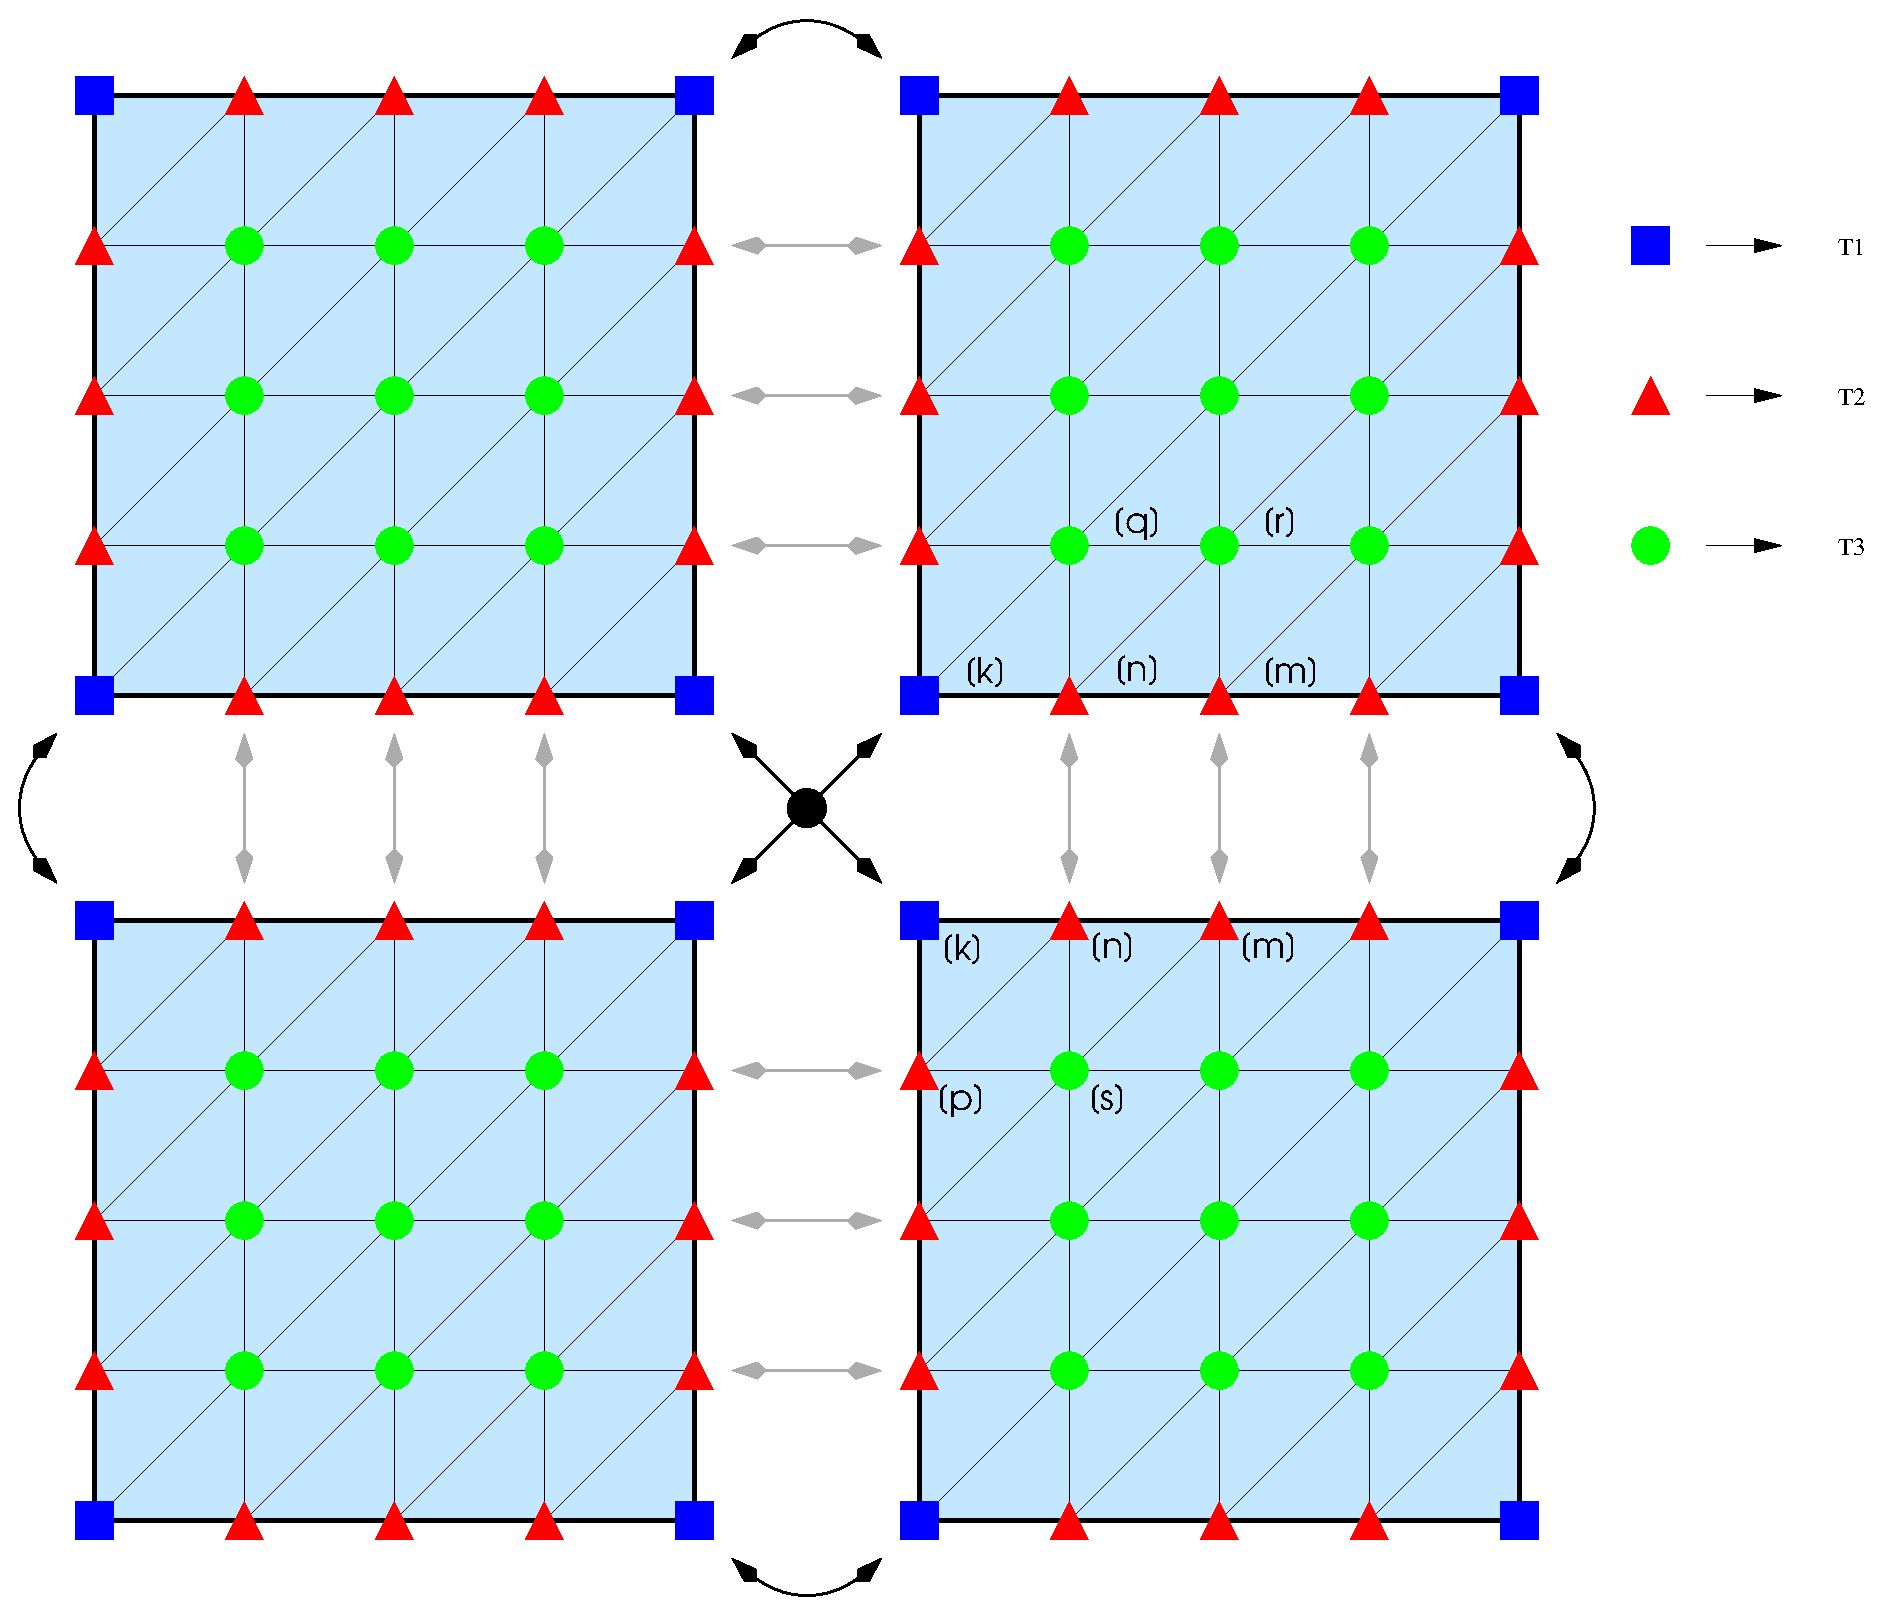
\includegraphics[width=0.4 \linewidth]{Grafiken/decomp.eps}
\end{center}

\vspace*{80pt}

Prof. Dr. Stefan Funken  \\
Prof. Dr. Karsten Urban\\
M.Sc. Lewin Ernst \\
  \vspace{8pt}
  Institute for Numerical Mathematics
  
%\preface
\newpage
\vspace{-2cm}
Das vorliegende Manuskript beinhaltet die Ausarbeitungen der
Projekte im Rahmen der Vorlesung High Performance Computing 2, 
welches im Sommersemester 2020 an der Fakult\"at f\"ur 
Mathematik und Wirtschaftswissenschaften der Universit\"at Ulm 
stattgefunden hat.

\medskip

Bedanken m\"ochten wir uns an dieser Stelle nochmals bei allen Teilnehmern f\"ur
ihre tollen Beitr\"age und gelungenen Vortr\"age, welche alle zusammen wesentlich 
zum Gelingen der Veranstaltung beigetragen haben.

\bigskip
\bigskip

Ulm, 2020 \hfill  Stefan Funken, Karsten Urban, Constantin Greif

  
  
  
 

\end{flushright}
\thispagestyle{empty} 

\newpage
\title{Incomplete Cholesky}
\author{Benjamin Bestler, Joachim Kr\"oner, Sebastian Acerbi}
\thispagestyle{empty} 

\maketitle
\tableofcontents

%%%%%%%%%%%%%%%%%%%%%%%%%%%%%%%%%%%%%%%%%%%%%%%%%

\section{Einleitung}
% Problembeschreibung
Partielle Differentialgleichungen stellen eine der h\"aufigsten Quellen f\"ur Probleme mit d\"unnbesetzten Matrizen dar. Eine typische Vorgehensweise ist die Diskrektrisierung der Gleichungen mit einer finiten Anzahl an Unbekannten. Die hierdurch entstehenden Gleichungssysteme sind meist sehr gro\ss, d\"unnbesetzt und oftmals symmetrisch positiv definit.\cite{saad03:IMS}


% Welche Arten von Lösern kommen in Frage(cg)
Als L\"osungsmethoden f\"ur solche Probleme k\"onnen sich klassische direkte L\"oser  als nicht praktikabel erweisen. Diese nutzen die spezielle Struktur der Matrix nicht aus, und k\"onnen sogar zu dicht besetzen Zerlegungen f\"uhren. 
Als geeigneter stellen sich iterative Methoden heraus, die sich schrittweise der optimalen L\"osung ann\"ahern, heraus. Ein bew\"ahrtes Verfahren dieser Klasse ist das konjugierte Gradientenverfahren, welches für  symmetrisch positiv definitite Matrizen anwendbar ist. Die anspruchvollste Operation stellt hier das Matrix-Vektor Produkt dar. Dieses kann f\"ur d\"unnbesetze Matrizen mit einem g\"unstigen Aufwand berechnet werden. \cite{GoluVanl96}

% Warum Vorkonditionierung
Allerdings weisen iterative Verfahren, wie das cg-Verfahren, eine geringere Robustheit als direkte Verfahren auf. Au{\ss}erdem h\"angt die Konvergenzgeschwindigkeit von der Kondition der Matrix ab. Bei Problemen, die sich aus typischen Anwendungen wie der Str\"umungsdynamik oder der Festigkeits- und Verformungsanalyse ergeben, kann dies zu einer langsamen Konvergenz führen.
Die Effizienz sowohl als die Robustheit k\"onnen jedoch signifikant durch geeignete Vorkonditionierung signifikant verbessert werden. \cite{saad03:IMS}

Die Wahl eines Vorkonditionierers hängt stark von den Eigenschaften der Matrix ab, weshalb die Wahl eines geeigneten Vorkonditionierers nicht leich ist. W\"ahrend direkte L\"osungsverfahren zur L\"osung von großen und d\"unnbesetzten Gleichungssystemen oft nicht anwendbar sind, stellen sie in modifizierter Form geeignete Vorkonditionierer für iterative Verfahren dar. Für

% Inhalt der Arbeit
Im Rahmen der Arbeit werden eine Auswahl an Verfahren zur Vorkonditionierung des konjugierten Gradientenverfahrens vorgestellt und verglichen. Folgende Verfahren wurden als Vorkonditionierer angewendet: Jacob-Verfahren, Gauss-Seidel, multigrid, Incomplete Cholesky und  INCE(0).

\newpage

Hier noch ein Algorithmus:

\begin{algorithm}[ht]
\caption{Variable metric hybrid inexact proximal point
method}\label{SG_alg:vmhippm}
\begin{algorithmic}[1]
\Function{Vmhippm}{$f, s, z^0$}
 \State $k \gets 0$
 \While{$k < k_{\max}$}
   \State $(u^k, g^k, \epsilon_k) \coloneqq \Call{Bundle}{f, s, M_k,
z^k, \delta_k}$ \Comment{Approximate the proximal point}
\If{$\frac{1}{2} \norm{g^k}^2 \le \rho\ \land\ \epsilon_k \le \rho$}
\State \Return $u^k$ \Comment{Optimal or close to optimal} \EndIf
   \State $z^{k+1} \coloneqq u^k$ \Comment{Step to the proximal point}
   \State $k \gets k + 1$
 \EndWhile
\EndFunction
\end{algorithmic}
\end{algorithm}

%Referenz: In Algorithmus \ref{SG_alg:vmhippm}.


Hier noch ein Code: 
\lstinputlisting{./ProjectX/Code/HelloWorld.c}



\begin{thebibliography}{2}
\bibitem{SG_Ben-Tal:2000}{\sc A. Ben-Tal, M. Kocvara, A.
Nemirovski, J. Zowe}: Free Material Design via Semidefinit
Programming, SIAM Review, Vol. 42, No. 4 (2000), 695-715.
\bibitem{saad03:IMS}{\sc Saad, Yousef} : Iterative Methods for Sparse Linear Systems, SIAM, Second Edition, (2003).
\bibitem{GoluVanl96}{\sc Golub, Gene H. and Van Loan, Charles F.} : Matric Computations, The Johns Hopkins University Press, Third Edition, (1996).
\end{thebibliography}


\end{document}